%% Beamer Presentation using 16:9 aspect ratio (HDTV standard aspect ratio)
\documentclass[aspectratio=169]{beamer}

%% Metropolis or mtheme Theme
\usetheme{metropolis}

% Packages
\usepackage{fancyvrb}
\usepackage{graphicx}
\usepackage{listings}
\usepackage[]{hyperref, amsmath}
\usepackage{pgfplots}
\usepackage{appendixnumberbeamer}
\usepackage{enumitem}
\usepackage[caption=false]{subfig}
\usepgfplotslibrary{statistics}
%\usepgfplotslibrary{external} 
%\tikzexternalize

% Provide an easy command for mono spaced font: \t{text}
\renewcommand{\t}[1]{\texttt{#1}}

% Provide an easy command for full screen graphics
\newcommand<>{\fullsizegraphic}[1]{
{
    \begin{frame}[plain]
        \begin{tikzpicture}[remember picture,overlay]
            \node[at=(current page.center)] {
                \includegraphics[width=\paperwidth]{#1}
            };
        \end{tikzpicture}
    \end{frame}
}
}
\newcommand<>{\fullsizegraphich}[1]{
{
    \begin{frame}[plain]
        \begin{tikzpicture}[remember picture,overlay]
            \node[at=(current page.center)] {
                \includegraphics[height=\paperheight]{#1}
            };
        \end{tikzpicture}
    \end{frame}
}
}

% Customize the Fancy Verbatim environment's default font and margins
\RecustomVerbatimEnvironment
{Verbatim}{Verbatim}
{formatcom=\scriptsize,xleftmargin=0.75ex}

% use filled blocks for default, alert and example blocks
\metroset{block=fill}

% Title format uses smallcaps
\metroset{titleformat=smallcaps}

% 42 Lines logo colors
\definecolor{blue}{RGB}{5,76,111}
\definecolor{lightblue}{RGB}{53,137,175}
\definecolor{grey}{RGB}{187,187,187}

% Adjust Metropolis theme to use 42 Lines colors
\setbeamercolor{alerted text}{fg=lightblue}
\setbeamercolor{example text}{fg=blue}
\setbeamercolor{palette primary}{bg=blue}

% Customization for code listings including font size, a background and margins
\lstset{
    basicstyle=\tiny\ttfamily,
    backgroundcolor=\color{normal text.bg!80!normal text.fg!50!normal text.bg},
    frame=single,
    framerule=0pt,
}

% Here ends the preamble


\title{Observability Data Engineering}
\subtitle{A Story About Math, Four Golden Signals, and Business Intelligence}
\institute{DevOps Observability Architect}
\author{Jack Neely\\ jjneely@gmail.com}

\date{\today}

\newcommand{\hcancel}[1]{%
    \tikz[baseline=(tocancel.base)]{%
        \node[inner sep=0pt,outer sep=0pt] (tocancel) {#1};
        \draw[red, very thick] (tocancel.south west) -- (tocancel.north east);
    }%
}%
\newcommand{\icancel}[1]{%
    \tikz[baseline=(tocancel.base)]{%
        \node[inner sep=0pt,outer sep=0pt] (tocancel) {#1};
        \draw[red, very thick] (tocancel.south west) -- (tocancel.north east);
        \draw[red, very thick] (tocancel.south east) -- (tocancel.north west);
    }%
}%

\usepackage[most]{tcolorbox}
\newtcolorbox{quotebox}{
    lower separated=false,
    arc=0pt,boxrule=0pt,leftrule=2pt
}

\begin{document}

%% Introduction, Title
\maketitle

%% In the Before Time Lightning Talk
%% Consultant work
%%\begin{frame}
%%    \frametitle{Monitorama PDX 2019: How to know if something is ``up''}
%%    \begin{tikzpicture}[remember picture,overlay]
%%        %%\node[at=(current page.center)] {
%%        %%    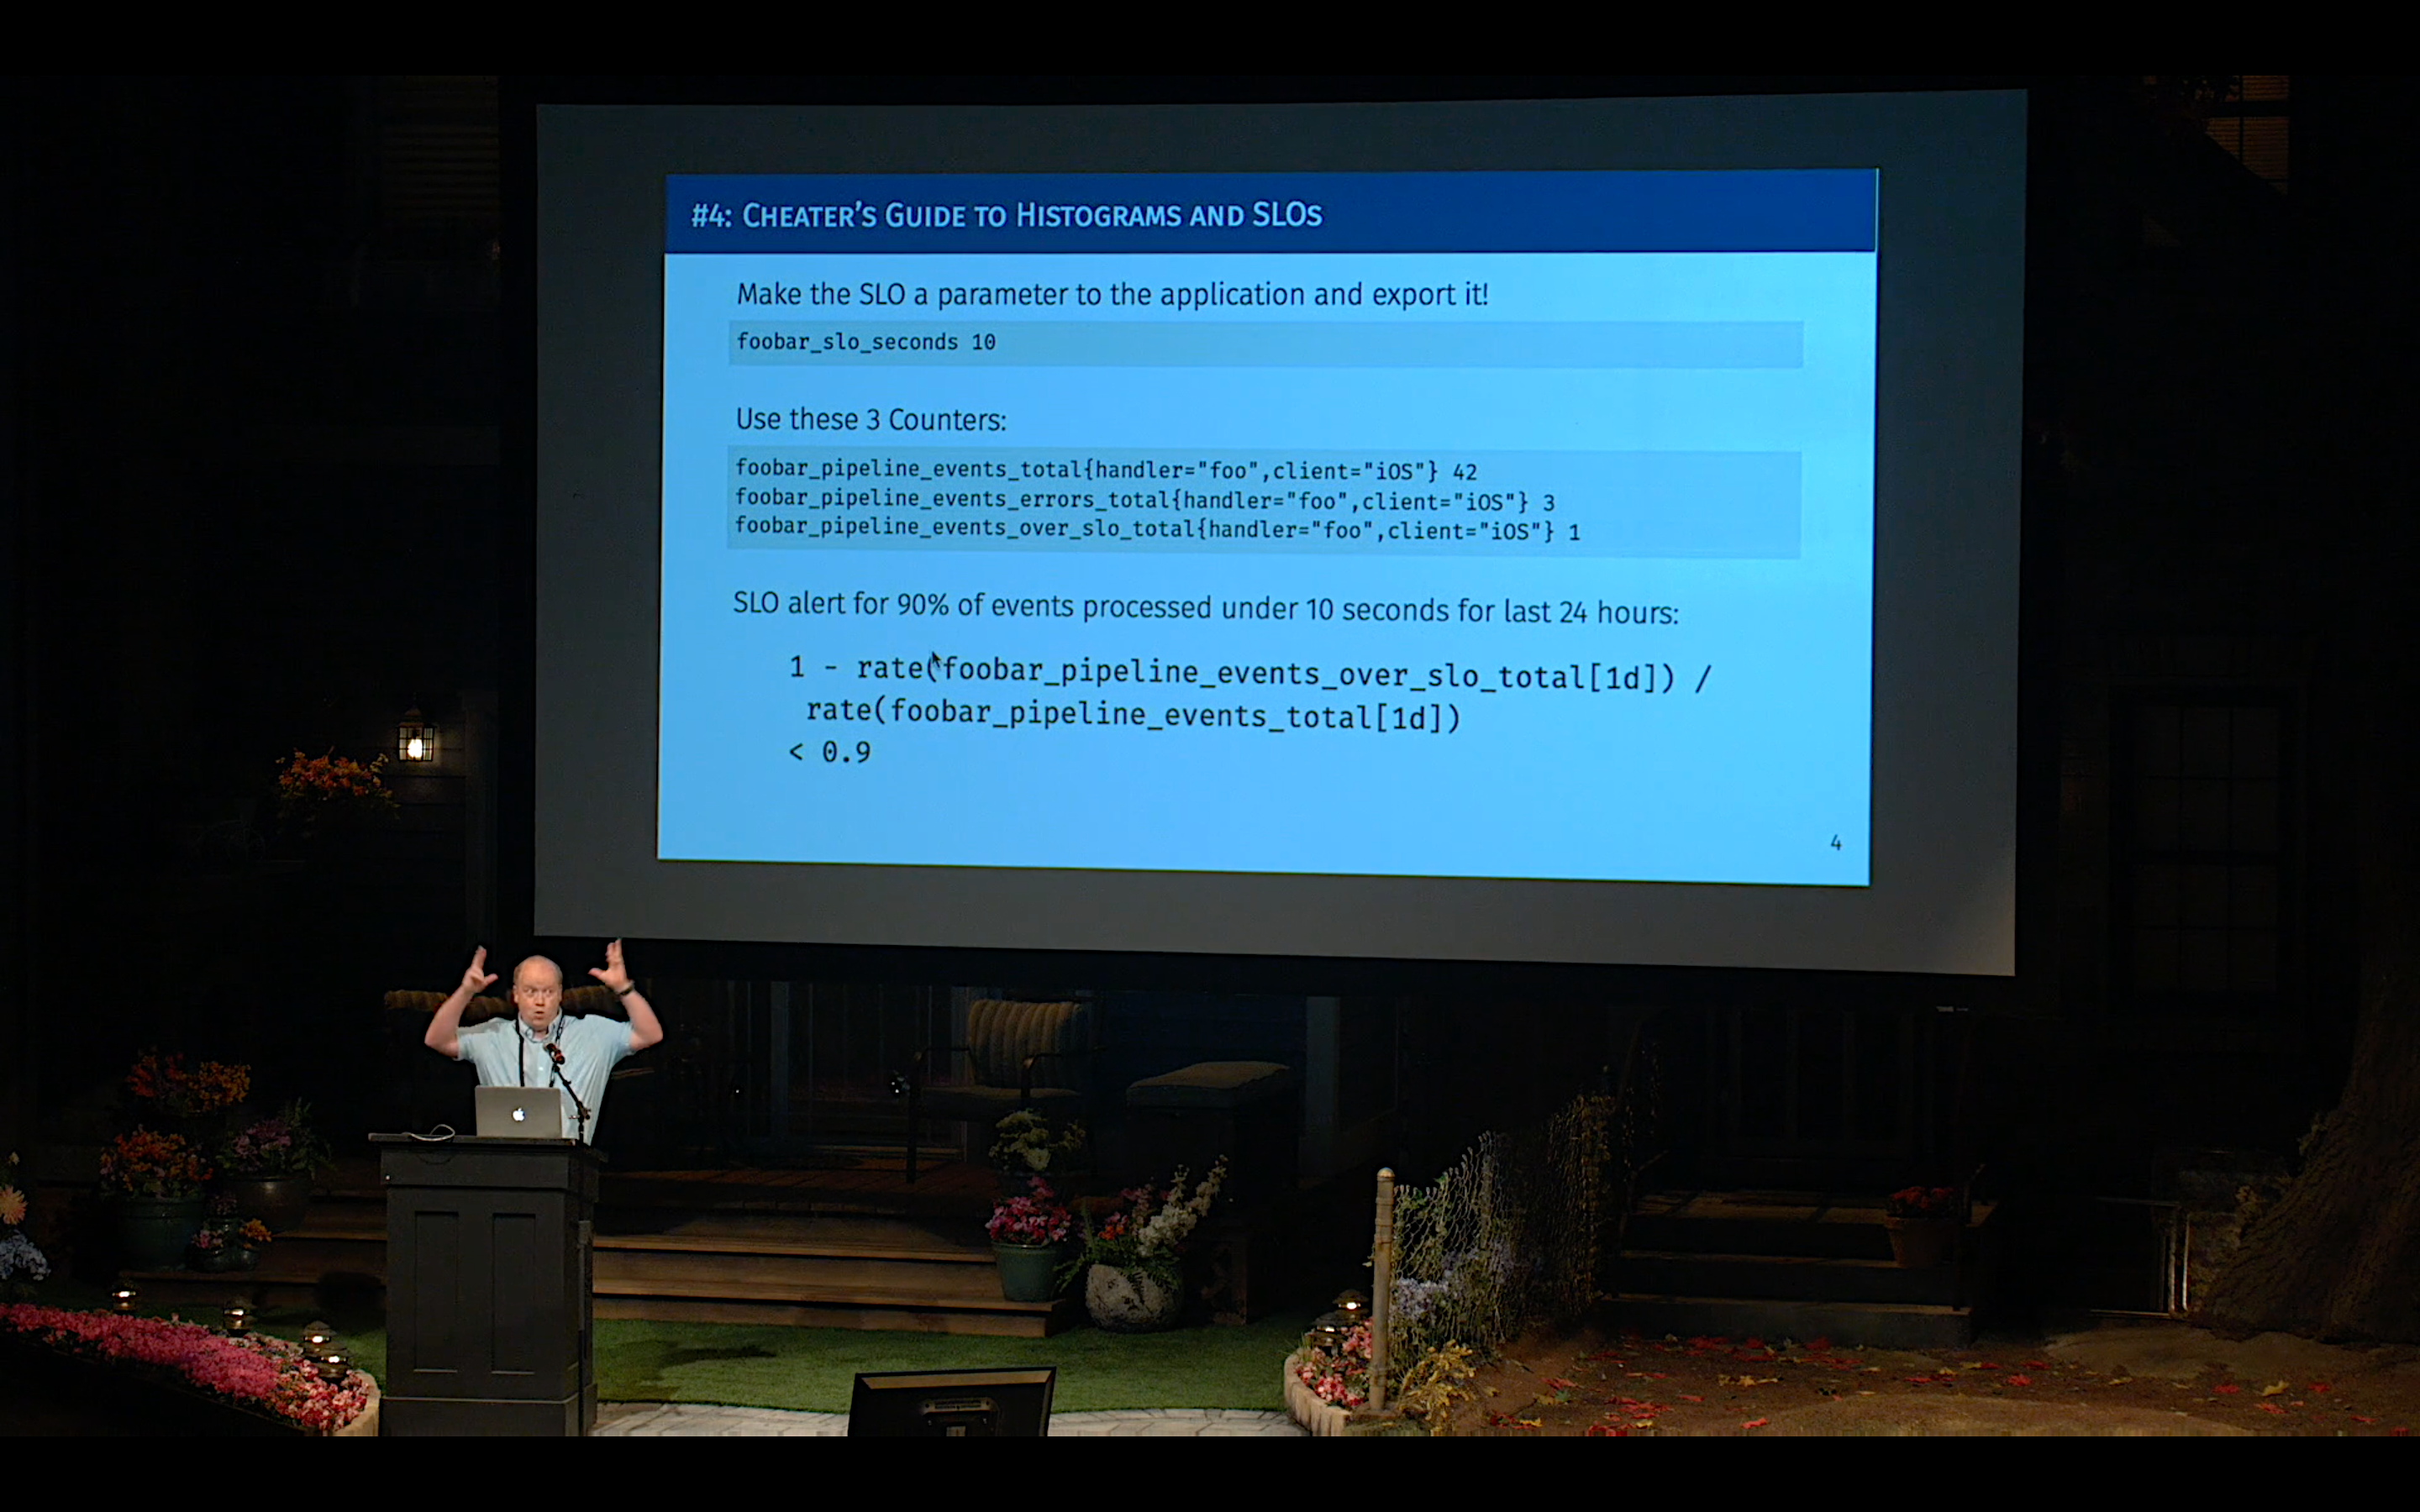
\includegraphics[width=10cm]{img/lightning-2019.png}
%%        %%};
%%    \end{tikzpicture}
%%\end{frame}

\begin{frame}
    \frametitle{As a DevOps Observability Architect...}

    \begin{quotebox}
    \emph{What do I monitor?}
    \end{quotebox}

    Google SRE's \hcancel{Four} Five Golden Signals
    \begin{description}[labelwidth=\widthof{Saturation}]
        \item[Traffic] Counter of Units of Work
        \item[Errors] Counter of Units of Work with Exceptions
        \item[Latency] Timer of the distribution of latencies for each Unit of Work
        \item[Saturation] When Pods be scaled up or down
        \item[Health] Is the thing up?  Does it respond to customers?
    \end{description}
\end{frame}

\begin{frame}
    \frametitle{As a DevOps Observability Architect...}

    The \icancel{Four} Five Golden Signals is knowing before the customers do.

    \begin{quotebox}
        \emph{We need to set alerts for these super special customers.}
    \end{quotebox}

    Well, if we set our Histograms correctly and record maximum values we will
    be able to tell when...

    \begin{quotebox}
        \emph{When a customer calls we need to be able to verify the error
            they encountered.  We'll need a high cardinally solution.}
    \end{quotebox}

    Umm...those aren't metrics.  Where are your traces?

    \begin{quotebox}
        \emph{Jack, we're an Enterprise!}
    \end{quotebox}
\end{frame}

\fullsizegraphic{img/enterprise-d-picard-309.png}

\begin{frame}[standout]
    Traffic

    \small{Why we count things}
\end{frame}

%% Count Units of Work
%% Why Counting monotonoically matters like a network device

\begin{frame}
    \frametitle{Why Counters Work}

    \begin{quotebox}
         Systems based in cumulative monotonic sums are naturally simpler, in
         terms of the cost of adding reliability. When collection fails
         intermittently, gaps in the data are naturally averaged from
         cumulative measurements.
         \tcblower
         \hfill --- OpenTelemetry Data Model Specification
    \end{quotebox}

    \begin{description}[labelwidth=\widthof{Synchronization}]
        \item[Accurate] Incremented in discrete whole numbers.  Never misses an event.
        \item[Synchronization] Primitive that allows for multiple observers.
        \item[Low Overhead] Easy implementation.  No copying or recalling previous values.
        \item[Fundamental] Position at time $t$.
    \end{description}

    %% https://www.researchgate.net/publication/3849082_Monotonic_counters_A_new_mechanism_for_thread_synchronization
\end{frame}

\begin{frame}
    \frametitle{Remembering Physics: First and Second Derivatives}
    \begin{columns}
        \begin{column}{0.33\textwidth}
            \begin{figure}[h!]
                \resizebox{\columnwidth}{!}{\begin{tikzpicture}[/pgf/declare function={f=3*x^3-6*x^2+2*x-1;}]
\begin{axis}[
    domain=0:10,
    ymax=2500,
    samples=100,
    axis lines=middle,
    xticklabel=$t_{\pgfmathprintnumber{\tick}}$
]
\addplot [thick] {f};
\end{axis}
\end{tikzpicture}
}
                \caption{Position: \scriptsize\tt{requests\_total}}
            \end{figure}
        \end{column}
        \begin{column}{0.33\textwidth}
            \begin{figure}[h!]
                \resizebox{\columnwidth}{!}{\begin{tikzpicture}[/pgf/declare function={f=9*x^2 - 12*x + 2;}]
\begin{axis}[
    domain=0:10,
    ymax=2500,
    samples=100,
    axis lines=middle,
    xticklabel=$t_{\pgfmathprintnumber{\tick}}$
]
\addplot [thick] {f};
\end{axis}
\end{tikzpicture}
}
                \caption{Velocity: \scriptsize\tt{rate(requests\_total[5m])}}
            \end{figure}
        \end{column}
        \begin{column}{0.33\textwidth}
            \begin{figure}[h!]
                \resizebox{\columnwidth}{!}{\begin{tikzpicture}[/pgf/declare function={f=18*x - 12;}]
\begin{axis}[
    domain=0:10,
    ymax=2500,
    samples=100,
    axis lines=middle,
    xticklabel=$t_{\pgfmathprintnumber{\tick}}$
]
\addplot [thick] {f};
\end{axis}
\end{tikzpicture}
}
                \caption{Acceleration: \scriptsize\tt{deriv(requests:rate5m[5m])}}
            \end{figure}
        \end{column}
    \end{columns}
    \note[item]{Spike detection}
\end{frame}

\begin{frame}[fragile]
    \frametitle{Counting Caveats: Riemann Sums}
    \note[item]{How to aggregate Counters}
    \begin{columns}
        \begin{column}{0.5\textwidth}
            \resizebox{\columnwidth}{!}{\pgfplotsset{
    integral segments/.code={\pgfmathsetmacro\integralsegments{#1}},
    integral segments=10,
    integral/.style args={#1:#2}{
        ybar interval,
        domain=#1+((#2-#1)/\integralsegments)/2:#2+((#2-#1)/\integralsegments)/2,
        samples=\integralsegments+1,
        x filter/.code=\pgfmathparse{\pgfmathresult-((#2-#1)/\integralsegments)/2}
    }
}

%% https://math.dartmouth.edu/opencalc2/cole/lecture8.pdf
%%\begin{tikzpicture}[/pgf/declare function={f=0.1*x^2+1;}]
\begin{tikzpicture}[/pgf/declare function={f=3*x^3-6*x^2+2*x-1;}]
\begin{axis}[
    domain=0:10,
    samples=100,
    axis lines=middle,
    xticklabel=$t_{\pgfmathprintnumber{\tick}}$
]
\addplot [
    red,
    fill=red!50,
    integral=0:10
] {f};
\addplot [thick] {f};
\end{axis}
\end{tikzpicture}
}
        \end{column}
        \begin{column}{0.5\textwidth}
\begin{lstlisting}
interval: 5m
rules:
- record: labels:http_server_requests:rate5m
  expr: >
    sum by (service, namespace, status) (
      rate(http_server_requests_seconds_count{}[5m])
    )
\end{lstlisting}

Integrate and Build Ratio:
            \begin{lstlisting}
1 - (
  sum_over_time(
    sum without (status) (
      labels:http_server_requests:rate5m{
        status=~"5..", service="..."})[7d:5m]
  ) * 300 /
  sum_over_time(
    sum without (status) (
      labels:http_server_requests:rate5m{
        service="..."})[7d:5m]
  ) * 300
)
            \end{lstlisting}
        \end{column}
    \end{columns}
\end{frame}

\begin{frame}[standout]
    Errors

    \small
    Your CPU Metrics are Wrong and I can Prove It
\end{frame}

%% Count Units of Work that fail or create an exception
%% How you CPU metrics are wrong

\begin{frame}[fragile]
    \frametitle{Measuring CPU Usage Over Time}

    How do you measure CPU usage of a process?
    \begin{enumerate}[label=\alph*.]
        \item Jiffies
        \item Percentages
        \item Seconds a Process is in the Running State
        \item All of the above
    \end{enumerate}
\end{frame}

\begin{frame}
    \frametitle{Nyquist-Shannon Sampling Theorem}
    \begin{figure}[!h]
        \centering
        \begin{tikzpicture}[/pgf/declare function={f=sin(deg(0.5*pi*x+0.25*pi));g=sin(deg(pi*x));}]
\begin{axis}[
    width=\textwidth,
    height=0.6\textheight,
    domain=0:10,
    samples=500,
    axis lines=middle,
    xticklabel=$t_{\pgfmathprintnumber{\tick}}$
]
\addplot [red, thick] {g};
    \addplot [mark=*, only marks] coordinates {(0.5,1) (4.5, 1) (8.5,1) (1.83, -0.5) (3.16,-0.5) (5.83,-0.5) (7.16,-0.5) (9.83,-0.5)};
\end{axis}
\end{tikzpicture}

    \end{figure}
    $$ Scrape Interval > 2f $$
\end{frame}
\begin{frame}
    \frametitle{Nyquist-Shannon Sampling Theorem: Aliasing}
    \begin{figure}[!h]
        \centering
        \begin{tikzpicture}[/pgf/declare function={f=sin(deg(0.5*pi*x+0.25*pi));g=sin(deg(pi*x));}]
\begin{axis}[
    width=\textwidth,
    height=0.6\textheight,
    domain=0:10,
    samples=500,
    axis lines=middle,
    xticklabel=$t_{\pgfmathprintnumber{\tick}}$
]
\addplot [dashed, thick] {f};
\addplot [red, thick] {g};
    \addplot [mark=*, only marks] coordinates {(0.5,1) (4.5, 1) (8.5,1) (1.83, -0.5) (3.16,-0.5) (5.83,-0.5) (7.16,-0.5) (9.83,-0.5)};
\end{axis}
\end{tikzpicture}

    \end{figure}
    $$ Scrape Interval > 2f $$
\end{frame}

\begin{frame}[standout]
    Latency

    \small
    And Other Non-Normal Distributions
\end{frame}

%% Latency: Timers and Distributions -- Why averages are horrible and
%% Anscombe's Quartet. Understanding Gamma Distributions.

\begin{frame}
    \frametitle{Anscomb's Quartet}
    \begin{columns}
        \begin{column}{0.3\textwidth}
            \begin{center}
                \begin{tabular}{ c c }
                    \multicolumn{2}{c}{\textbf{Summary Statistics}} \\
                    \hline
                    $N$ & $11$ \\
                    $\mu\{x_1..x_n\}$ & $9.0$ \\
                    $\mu\{y_1..y_n\}$ & $7.5$ \\
                    $\sigma\{x_1..x_n\}$ & $3.16$ \\
                    $\sigma\{y_1..y_n\}$ & $1.94$ \\
                    $r^2$ & $0.67$
                \end{tabular}
            \end{center}
        \end{column}
        \begin{column}{0.7\textwidth}
            \begin{figure}[!h]
                \centering
                \subfloat{%
\begin{tikzpicture}[/pgf/declare function={f=0.5001*x+3.0001;}]
\begin{axis}[
    %%width=\textwidth,
    height=4.5cm,
    xmax=20,
    xmin=0,
    ymin=0,
    ymax=13,
    samples=100,
    domain=0:20,
    axis lines=middle,
    yticklabels={,,},
    xticklabels={,,},
    mark size=1pt,
]
    \addplot [mark=*, only marks] table[x=x1, y=y1] {anscombs.dat};
    \addplot [red] {f};
\end{axis}
\end{tikzpicture}%
}%
%
\subfloat{%
\begin{tikzpicture}[/pgf/declare function={f=0.5000*x+3.0009;}]
\begin{axis}[
    %%width=\textwidth,
    height=4.5cm,
    xmax=20,
    xmin=0,
    ymin=0,
    ymax=13,
    samples=100,
    domain=0:20,
    axis lines=middle,
    yticklabels={,,},
    xticklabels={,,},
    mark size=1pt,
]
    \addplot [mark=*, only marks] table[x=x2, y=y2] {anscombs.dat};
    \addplot [red] {f};
\end{axis}
\end{tikzpicture}%
}

\subfloat{%
\begin{tikzpicture}[/pgf/declare function={f=0.4997*x+3.0025;}]
\begin{axis}[
    %%width=\textwidth,
    height=4.5cm,
    xmax=20,
    xmin=0,
    ymin=0,
    ymax=13,
    samples=100,
    domain=0:20,
    axis lines=middle,
    yticklabels={,,},
    xticklabels={,,},
    mark size=1pt,
]
    \addplot [mark=*, only marks] table[x=x3, y=y3] {anscombs.dat};
    \addplot [red] {f};
\end{axis}
\end{tikzpicture}%
}%
%
\subfloat{%
    \begin{tikzpicture}[/pgf/declare function={f=0.4999*x+3.0017;}]
\begin{axis}[
    %%width=\textwidth,
    height=4.5cm,
    xmax=20,
    xmin=0,
    ymin=0,
    ymax=13,
    samples=100,
    domain=0:20,
    axis lines=middle,
    yticklabels={,,},
    xticklabels={,,},
    mark size=1pt,
]
    \addplot [mark=*, only marks] table[x=x4, y=y4] {anscombs.dat};
    \addplot [red] {f};
\end{axis}
\end{tikzpicture}%
}

            \end{figure}
        \end{column}
    \end{columns}
\end{frame}

% Show overlay of Standard Distribution on top of real latency data
\begin{frame}
    \frametitle{Nonstandard Distributions}
    \begin{figure}[!h]
        \centering
        \begin{tikzpicture}[/pgf/declare function={sigma=1; mu=1; f=(1/(sigma*sqrt(2*pi)))*e^(-((x-mu)^2)/(2*sigma^2));}]
\begin{axis}[
    %%width=\textwidth,
    %%height=0.6\textheight,
    ymax=0.5,
    domain=-6:6,
    samples=500,
    axis lines=middle,
    xticklabel=$t_{\pgfmathprintnumber{\tick}}$
]
\addplot [red, thick] {f};
\end{axis}
\end{tikzpicture}

    \end{figure}
\end{frame}
\begin{frame}
    \frametitle{Nonstandard Distributions}
    \begin{figure}[!h]
        \centering
        \begin{tikzpicture}[/pgf/declare function={sigma=0.7330352; mu=0.2902809; f=(1/(sigma*sqrt(2*pi)))*e^(-((x-mu)^2)/(2*sigma^2));}]
\begin{axis}[
    width=15cm,
    height=7.5cm,
    %%domain=-6:6,
    xmax=8,
    xmin=-4,
    samples=500,
    axis lines=middle,
    xticklabel=$t_{\pgfmathprintnumber{\tick}}$,
    bar width=3pt,
    ylabel=Density
]
\addplot [ybar, color=blue, fill=blue!50] table[x index=0, y index=1]{graphite-hist.dat};
\node[circle,fill=blue,scale=0.5,pin=45:{Actual $p997$}] at (axis cs:3.172055554,0.01) {};
    \node (A) at (axis cs:5,0.5) {Last Observation at $t_{29}$};
    \draw[->] (A) to (axis cs:8,0.5);
\addplot [red, thick] {f};
\node[circle,fill=red,scale=0.5,pin=45:{$3\sigma$}] at (axis cs:2.1991,0.01) {};
\end{axis}
\end{tikzpicture}

    \end{figure}
\end{frame}

\begin{frame}
    \frametitle{Standard Distribution Curve Formula}

    {\huge $$ f(x) = \frac{1}{\sigma \sqrt{2\pi}} e^{-\frac{(x-\mu)^2}{2\sigma^2}} $$ }

    \vskip 1em
    \begin{description}
        \item[$\sigma$] Standard Deviation
        \item[$\mu$] Mean
        \item[$e$] The base of the Natural Logarithm, about $2.71828$
        \item[$\pi$] Pi!
    \end{description}
\end{frame}

\begin{frame}[standout]
    Saturation

    \small
    Are You Saturated Yet?
\end{frame}

%% Saturation: Percentiles and Pipelines -- Visualizing percentiles of data,
%% why we cannot combine percentiles, and the magic of histograms.
\tikzstyle{process} = [
    rectangle,
    minimum width=2.5cm, 
    minimum height=0.75cm,
    text centered, 
    draw=black, 
    fill=white,
]
\tikzstyle{textstyle} = [
    rectangle,
    align=left,
    minimum width=1.5cm, 
    minimum height=0.75cm,
]
\tikzstyle{arrow} = [
    thick,
    ->,
    >=stealth
]

\newcommand\pipelinetikz{
    %%\draw[step=1cm,gray,very thin] (0,0) grid (15,-6);
    \node (stage1) [textstyle] {Stage 1\\Pod A};
    \node (stage2) [textstyle, below of=stage1] {Stage 2\\Pod B};
    \node (stage3) [textstyle, below of=stage2] {Stage 3\\Pod C};
    \node (otel1) [textstyle, right of=stage1, xshift=14cm] {OTEL};
    \node (otel2) [textstyle, right of=stage2, xshift=14cm] {OTEL};
    \node (otel3) [textstyle, right of=stage3, xshift=14cm] {OTEL};
    \draw [arrow,dashed] (stage1) -- (otel1);
    \draw [arrow,dashed] (stage2) -- (otel2);
    \draw [arrow,dashed] (stage3) -- (otel3);
    \node (job1) [process, right of=stage1, xshift=1.5cm] {Job};
    \node (job2) [process, right of=stage2, xshift=5cm] {Job};
    \node (job3) [process, right of=stage3, xshift=8.5cm] {Job};
    \node (job4) [process, right of=job3, xshift=1cm] {Job};
    \draw [arrow] (job1) -- (3.5,-1) -- node[anchor=north east] {Queue Time} (7,-1) -- (job2);
    \draw [arrow] (job2) -- (7, -3) -- node[anchor=north east] {Queue Time} (10.5, -3) -- (job3);
    \draw [arrow] (job2) -- (7, -3) -- (13.5, -3) -- (job4);
}

\begin{frame}
    \frametitle{Tracing Pipelines}
    \centering
    \resizebox{\textwidth}{!}{%
    \begin{tikzpicture}[node distance=2cm]
        \pipelinetikz
        %%\draw [draw=red, thick] (2,0.5) rectangle (15,-4.5);
    \end{tikzpicture}}
    \raggedright

    \begin{description}
        \item[Freshness SLO]  X\% of results are processed in Y time or less over the last Z days.
        \item[Saturation SLO] X\% of results have Y queue time or less over the last Z days.
    \end{description}
    \note[item]{Jobs may take hours}
    \note[item]{Jobs may fan out or reduce}
    \note[item]{There is no root span}
\end{frame}

\begin{frame}
    \frametitle{Tracing Pipelines: How to FAIL}
    \centering
    \resizebox{\textwidth}{!}{%
    \begin{tikzpicture}[node distance=2cm]
        \pipelinetikz
        \draw [draw=red, thick] (2,0.5) node[anchor=south west, color=red] {TraceId: DEADBEEF} rectangle (15,-4.5);
    \end{tikzpicture}}
\end{frame}

\tikzstyle{process} = [
    rectangle,
    minimum width=2.5cm, 
    minimum height=0.75cm,
    text centered, 
    draw=red, 
    fill=white,
]
\begin{frame}
    \frametitle{Tracing Pipelines: Using Span Links}
    \centering
    \resizebox{\textwidth}{!}{%
    \begin{tikzpicture}[node distance=2cm]
        \pipelinetikz
        \node [color=red, anchor=south] at (7,-1) {Span Link};
        \node [color=red, anchor=south] at (10.5,-3) {Span Link};
    \end{tikzpicture}}
    \raggedright

    Create a TraceId per job and pass context across the bus.  Child jobs
    create a Span Link to reference the TraceId of the parent pipeline job.
\end{frame}

\begin{frame}[fragile]
    \frametitle{Tracing Pipelines: KISS Method}

    Build a schema and pass meta information along the bus.
    \begin{figure}[h!]
        \begin{tabular}{c}
        \begin{lstlisting}[linewidth=5cm]
{
  custId        : int,
  discoveredTs  : Unix Epoch,

  stage1_traceId: string,
  stage1_status : int,
  stage1_startTs: Unix Epoch,
  stage1_stopTs : Unix Epoch,

  stage2_traceId: string,
  stage2_status : int,
  stage2_startTs: Unix Epoch,
  stage2_stopTs : Unix Epoch,

  stage3_traceId: string,
  stage3_status : int,
  stage3_startTs: Unix Epoch,
  stage3_stopTs : Unix Epoch
}
        \end{lstlisting}
        \end{tabular}
    \end{figure}
\end{frame}


\begin{frame}[standout]
    Health

    \small
    Of Your Customers
\end{frame}

%% T-Digests

\begin{frame}
    \frametitle{Mission Impossible}

    \textbf{Goal:} Per Customer Median and Percentiles

    \textbf{Problem:} High Velocity Log/Event Data
    \vskip 0.5cm
    \textbf{Goal:} Summarize Per Customer Data Every 15 Minutes

    \textbf{Problem:} Calculating 7 - 30 Day Percentiles from Rollups

    \vskip 0.5cm
    \centering\large
    \tt{\{ $ts$: 2023-06-08T22:15:00, $custId$: 9, $N$: 4, $\mu$: 581, $q(.99)$: 595 \}}

\end{frame}

\begin{frame}
    \frametitle{T-Digest}

    \begin{columns}
        \begin{column}{0.4\textwidth}

            $$ k(q) = \frac{\delta}{2\pi} \sin^{-1}(2q-1) $$
            ~
            \begin{description}
                \item[$q$] Quantile ($0 - 1$ Inclusive)
                \item[$k$]  Scale Factor
                \item[$\delta$] Compression Constant
                \item[$\pi$] Everybody run!  It's $\pi$ again!
            \end{description}
        \end{column}
        \begin{column}{0.6\textwidth}
            \begin{figure}[!h]
                \centering
                \resizebox{\columnwidth}{!}{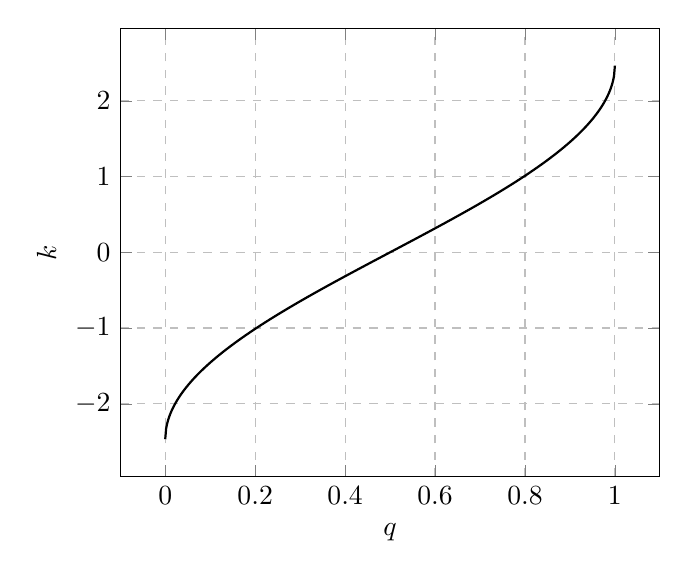
\begin{tikzpicture}[/pgf/declare function={f=(1/2*pi) * rad(asin(2*x-1));}]
\begin{axis}[
    domain=0:1,
    samples=500,
    xlabel=$q$,
    ylabel=$k$,
    grid style=dashed,
    ymajorgrids=true,
    xmajorgrids=true,
]
%%\addplot [thick] gnuplot[samples=100] {f};
\addplot [thick] {f};
\end{axis}
\end{tikzpicture}
}
            \end{figure}
        \end{column}
    \end{columns}
\end{frame}

\begin{frame}
    \frametitle{Results 24 Hour $q(.99)$ Estimations from 15 Minute Rollups}
    Results: 80/20 Rule.  

    \vskip 1em
    \begin{figure}[!h]
        \centering
        %% Extreme outlier plot
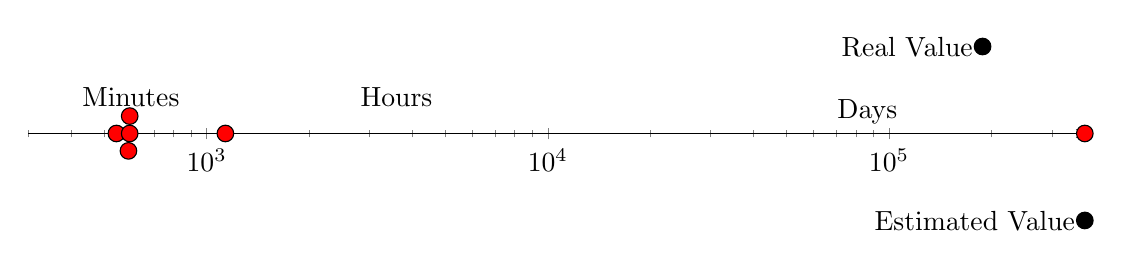
\begin{tikzpicture}
\begin{semilogxaxis}[
    axis x line=center,% only show the bottom x axis
    hide y axis,    
    ymin=-1,ymax=1,
    xmin=300,
    width=15cm,
    height=6cm,
    mark size=3pt,
]
\addplot[fill=red,only marks] table {%
544 0
590 -0.1
595 0.1
595 0
1135 0
374909 0
};
\addplot[fill=black, only marks] table {%
188022 0.5
374909 -0.5
};
\node[above] at (axis cs:3600,0.1) {Hours};
\node[above] at (axis cs:600,0.1) {Minutes};
\node[above] at (axis cs:86400,0) {Days};
\node[left] at (axis cs:188022,0.5) {Real Value};
\node[left] at (axis cs:374909,-0.5) {Estimated Value};
\end{semilogxaxis}
\end{tikzpicture}

        \caption{Example of High Error Customer Distribution}
    \end{figure}

    Adjusted Hypothesis: Serialized T-Digests as 15 minute rollups will have better accuracy.
    
    Results: 95\% of Customer $q(.99)$ Very Accurate
\end{frame}

\begin{frame}[standout]
    \small

    Averages Lie

    Use Smart Rollups

    There Are FIVE Golden Signals

    Use Quantiles and Max to Understand Latency Spread

    Use the Scientific Method and Mathematically Model Applications
\end{frame}

\begin{frame}[standout]
    Thank You!
    $$\pi$$

    \small
    Jack Neely
    jjneely@gmail.com

    Podcast: operations.fm
\end{frame}

\appendix

\begin{frame}
    \frametitle{References}

    \begin{itemize}
        \item Enterprise D Image Credit: PARAMOUNT
        \item T-Digests: \href{https://github.com/tdunning/t-digest}{https://github.com/tdunning/t-digest}
    \end{itemize}
\end{frame}
\end{document}
